\documentclass[sigconf]{acmart}

\setcopyright{none}
\settopmatter{printacmref=false}
\renewcommand\footnotetextcopyrightpermission[1]{}
\pagestyle{plain}

\usepackage{booktabs}
\usepackage{amssymb}
\usepackage{mathtools}

\newcommand{\R}{\mathbb{R}}
\newcommand{\concat}{\mathbin\Vert}
\newcommand{\conf}{\mathcal{C}_{\tau}}

\title{When Cross-View Helps Most: Conflict-Aware Disaster Triage Across Spatial Observation Regimes}

\author{Anonymous Author(s)}
\affiliation{%
  \institution{Anonymous Institution}
  \city{Anonymous City}
  \country{Anonymous Country}
}
\email{anonymous@example.com}

\begin{abstract}
Cross-view disaster assessment combines ground-level and overhead imagery to
infer building damage, but most prior work is still framed around average test
performance. That framing hides the cases in which multimodal fusion matters
most: samples where the single-view predictors disagree. We study cross-view
disaster triage through this conflict-centered lens on two paired datasets with
different spatial observation regimes: an Eaton/Altadena wildfire dataset built
from property-centric inspection imagery and paired overhead patches, and a
Hurricane Ian benchmark built from panoramic ground imagery and paired overhead
patches. We propose a Conflict-Aware Evaluation protocol (CAE) that reports
overall F1, conflict-subset F1 under a soft disagreement threshold, and the
conflict gain of cross-view fusion over the best single-view model. CAE shows
that cross-view fusion is most useful on evidence-conflict cases, but the
source and size of that gain depend on the ground-view regime. In wildfire
imagery, the ground view is the clearer single-view arbitrator. In hurricane
settings, the stronger single view becomes split-sensitive rather than
universally fixed, which argues for more careful regime-aware interpretation
than a simple disaster-name comparison. We further show that tile-level
cross-view conflict density forms an unsupervised spatial damage signal in the
wildfire dataset, and that a conflict-aware training objective improves
wildfire cross-view F1 from 0.9473 to 0.9520. Together, these results recast
cross-view disaster assessment from average-case multimodal classification to
conflict-aware, regime-aware spatial reasoning.
\end{abstract}

\keywords{disaster assessment, cross-view learning, multimodal fusion, GeoAI, conflict-aware evaluation}

\begin{document}

\maketitle

\section{Introduction}

Post-disaster building assessment increasingly relies on multiple visual
modalities. Overhead imagery provides broad geographic coverage and stable
spatial context, while ground-level imagery exposes facade condition,
street-facing damage, and local structural cues. Cross-view models are intended
to combine these complementary signals. In practice, however, most cross-view
studies still ask only whether multimodal fusion improves average performance.
That question is incomplete.

The more consequential question is when cross-view fusion actually matters. In
real deployments, many samples are easy. A heavily damaged building may be
obvious in both views, while an intact building may be equally clear from both
street and overhead imagery. Cross-view fusion becomes most valuable when the
two modalities provide competing evidence. Those disagreement cases are exactly
where a deployment team would most want an additional source of information or
a more reliable fusion policy.

This paper studies cross-view disaster triage from that perspective. We argue
that cross-view value is fundamentally conflict-dependent and regime-dependent.
It is conflict-dependent because the practical value of fusion is concentrated
in cases where single-view models disagree. It is regime-dependent because the
relative usefulness of ground and overhead evidence changes with the spatial
observation regime of the ground-view imagery. A property-centric inspection
photo and a panoramic environmental photo are both ground-view images, but they
encode very different relationships to the target building.

We investigate this hypothesis on two paired disaster datasets. The first is an
Eaton/Altadena wildfire dataset built from property-centric inspection imagery
paired with overhead patches. The second is a Hurricane Ian benchmark built
from panoramic ground imagery paired with overhead patches. These datasets do
not merely differ by disaster type. More importantly, they differ by spatial
observation regime: the wildfire ground view is usually tightly aligned with
the target property, whereas the hurricane ground view often contains broader
environmental context and weaker target alignment.

To study these settings, we introduce a Conflict-Aware Evaluation protocol
(CAE). CAE reports: (1) standard overall F1 on the full test set, (2)
Conflict-F1 on the subset of samples where the single-view models disagree
under a soft probability-gap threshold, and (3) the conflict gain of cross-view
fusion over the best single-view baseline. This protocol shifts the paper's
evaluation axis from average-case performance to conflict resolution.

Using CAE, we find that cross-view fusion is consistently strongest on
disagreement cases, but the dominant single view changes with the evaluation
setting. Wildfire is clearly street-dominant on conflict cases. Hurricane is
more nuanced: the endpoint split is close to balanced, while the broader label
sensitivity split becomes overhead-favoring. That difference matters because it
prevents overclaiming a simplistic ``wildfire versus hurricane'' story and
instead supports a more careful observation-regime interpretation.

We then show that the conflict-centered framing leads to two useful method
extensions. First, a tile-level conflict density map, computed from the
disagreement magnitude between street-only and remote-only predictors, becomes
a significant unsupervised spatial damage indicator in the wildfire dataset.
Second, a conflict-aware training objective, ConflictFocalLoss, improves
wildfire cross-view performance across multiple weighting settings, with the
best run increasing test F1 from 0.9473 to 0.9520.

This paper makes four main contributions:
\begin{enumerate}
  \item We introduce a Conflict-Aware Evaluation protocol for paired-view
  disaster triage, shifting evaluation from average-case F1 to conflict-centered
  reasoning.
  \item We show that cross-view gain is regime-dependent: wildfire is clearly
  street-dominant, while hurricane is more split-sensitive and therefore
  requires more careful interpretation than a single aggregate claim.
  \item We demonstrate that tile-level cross-view conflict density forms an
  unsupervised spatial damage map in the wildfire setting.
  \item We show that conflict-aware training can improve cross-view triage,
  with a complete ConflictFocalLoss sweep yielding consistent gains for
  moderate weighting levels.
\end{enumerate}

The broader implication is that cross-view disaster intelligence should not be
modeled as generic multimodal fusion. It should be understood as conflict-aware,
regime-aware spatial reasoning.

\section{Related Work}

Research on post-disaster visual assessment has largely focused on single-view
remote sensing benchmarks, especially satellite-only settings such as xBD
\cite{gupta2019xbd}. This literature has established strong baselines for
damage classification and mapping, but it does not address how different visual
viewpoints interact when they disagree.

A smaller body of work studies ground-view imagery for disaster assessment.
These approaches recover local structural evidence that overhead imagery cannot
directly observe, but ground-only models face their own limitations: narrow
viewpoint, occlusion, non-uniform coverage, and dependence on how well the
captured scene aligns with the target structure.

Recent cross-view disaster work begins to bridge these modalities. The closest
prior direction is CVDisaster, which studies cross-view geolocalization and
damage estimation for Hurricane Ian using paired street-view and very
high-resolution satellite imagery \cite{li2024cvdisaster}. That work
demonstrates that paired-view learning is feasible and useful, but it still
evaluates mainly by aggregate classification performance. It does not separate
easy cases from disagreement cases, and it does not ask whether the dominant
evidence source changes across spatial observation regimes.

More broadly, multimodal fusion in computer vision and geospatial learning
often assumes that modalities should be fused symmetrically. In disaster
settings, that assumption is fragile. A property-centric inspection image and a
panoramic environmental image carry different target alignment, different
spatial context, and different failure modes. Our work is closer in spirit to
GeoAI studies that ask how spatial observation processes shape model behavior,
rather than merely which architecture gives the highest average score.

This paper differs from prior cross-view disaster work in three ways. First, it
defines the conflict subset as the primary evaluation target. Second, it uses a
cross-regime design to compare two observation regimes rather than merely two
datasets. Third, it translates disagreement analysis into spatial and
algorithmic outputs: a conflict-density map, a conflict-aware training loss,
and an adaptive conflict-resolver view of cross-view inference.

\section{Problem Setting and Datasets}

\subsection{Task}

We study binary disaster triage from paired images. Each example contains a
ground-view image and a paired overhead patch, with a binary damage label. The
goal is to predict whether the target building belongs to the positive or
negative damage class under a specified split definition.

Formally, the evaluation set is
\begin{equation}
\mathcal{D}=\{(x_i^{(s)},x_i^{(r)},y_i)\}_{i=1}^{N},
\end{equation}
where $x_i^{(s)}$ is the street- or ground-view image,
$x_i^{(r)}$ is the remote-view overhead patch, and
$y_i\in\{0,1\}$ is the binary damage label. For a model $m$, let
$p_i^{(m)}\in[0,1]$ denote the predicted probability of the positive class and
$\hat{y}_i^{(m)}=\mathbf{1}[p_i^{(m)}\ge 0.5]$ its hard decision.

We consider three model settings under a shared training protocol:
\begin{itemize}
  \item \texttt{street\_only}: ground image only
  \item \texttt{remote\_only}: overhead image only
  \item \texttt{crossview}: paired ground plus overhead fusion
\end{itemize}

\subsection{Eaton/Altadena Wildfire Dataset}

Our wildfire dataset pairs property-centric inspection imagery with overhead
patches. The ground images are typically taken from close range and are
visually anchored to the target property. This gives the dataset strong target
alignment and makes it a natural setting to study whether local facade evidence
helps resolve conflicts in overhead interpretation.

For the primary wildfire binary triage task, we use:
\begin{itemize}
  \item \texttt{0 = No Damage + Affected}
  \item \texttt{1 = Minor + Major + Destroyed}
\end{itemize}

We also evaluate a stricter sensitivity split:
\begin{itemize}
  \item \texttt{0 = No Damage}
  \item \texttt{1 = Affected + Minor + Major + Destroyed}
\end{itemize}

The wildfire dataset additionally contains spatial grouping metadata, which
allows tile-level geographic analysis and map-based outputs.

\subsection{Hurricane Ian Benchmark}

The hurricane benchmark pairs panoramic ground imagery with overhead patches.
Unlike the wildfire dataset, the ground view here is not tightly centered on a
single property. It often includes broader street context, neighboring
structures, and environmental clutter. We therefore treat it as a panoramic or
environment-centric observation regime.

For the endpoint binary setting, we use:
\begin{itemize}
  \item \texttt{0 = MinorDamage}
  \item \texttt{1 = SevereDamage}
\end{itemize}

We also evaluate a broader sensitivity setting:
\begin{itemize}
  \item \texttt{0 = MinorDamage}
  \item \texttt{1 = ModerateDamage + SevereDamage}
\end{itemize}

The original hurricane endpoint split showed object-level leakage. We therefore
rebuilt a clean grouped split and use it as the more reliable hurricane control
condition.

\subsection{Why This Comparison Matters}

These datasets give us more than a two-disaster benchmark. They instantiate two
different spatial observation regimes:
\begin{itemize}
  \item building-centric / property-centric
  \item panoramic / environment-centric
\end{itemize}

This regime distinction is central to the paper. We do not assume cross-view
fusion is equally valuable in all paired-view settings. Instead, we test
whether its gain depends on how directly the ground-view image captures the
target structure.

\section{Conflict-Aware Evaluation Protocol}

Average test F1 is necessary but insufficient. To isolate the value of
cross-view fusion in the cases that matter most, we define a Conflict-Aware
Evaluation protocol (CAE).

For each completed setting, CAE reports:
\begin{enumerate}
  \item \textbf{Overall-F1}: standard F1 over the full test set.
  \item \textbf{Conflict-F1}: F1 over the disagreement subset defined by
  \texttt{|p\_street - p\_remote| > tau}.
  \item \textbf{Delta\_view}: the gain of cross-view fusion over the better
  single-view model on the conflict subset.
\end{enumerate}

In the main experiments, we use \texttt{tau = 0.1}. This soft conflict
definition is more robust than a hard binary disagreement test and yields
usable conflict-set sizes for both datasets. Under this definition, the
conflict subset contains 435 wildfire samples and 128 hurricane
moderate-plus-severe samples, both with label-independence permutation-test
significance below \texttt{1e-4}.

More precisely, the conflict subset is
\begin{equation}
\conf=\left\{i:\left|p_i^{(s)}-p_i^{(r)}\right|>\tau\right\},
\label{eq:conflictset}
\end{equation}
where $p_i^{(s)}$ and $p_i^{(r)}$ are the positive-class probabilities from
the street-only and remote-only models, respectively. For any model $m$ and
subset $\mathcal{S}\subseteq\{1,\dots,N\}$, we compute
\begin{equation}
\mathrm{F1}(m;\mathcal{S})=
\frac{2\,\mathrm{Prec}(m;\mathcal{S})\,\mathrm{Rec}(m;\mathcal{S})}
{\mathrm{Prec}(m;\mathcal{S})+\mathrm{Rec}(m;\mathcal{S})}.
\label{eq:f1}
\end{equation}
The conflict gain of cross-view fusion is then
\begin{equation}
\Delta_{\mathrm{view}}=
\mathrm{F1}(\mathrm{crossview};\conf)
-\max\left\{
\mathrm{F1}(\mathrm{street};\conf),
\mathrm{F1}(\mathrm{remote};\conf)
\right\}.
\label{eq:deltaview}
\end{equation}

Conceptually, CAE reframes the task. Instead of asking whether multimodal
fusion improves average classification, CAE asks whether fusion helps when the
single-view models disagree and which modality drives that improvement.

\begin{table*}[t]
  \caption{Conflict-Aware Evaluation (CAE) summary across completed settings.}
  \label{tab:cae}
  \centering
  \begin{tabular}{llrrrr}
    \toprule
    Setting & Mode & Overall-F1 & Conflict-F1 ($\tau=0.1$) & Delta\_view & $n_{\mathrm{conflict}}$ \\
    \midrule
    Wildfire sensitive & street\_only & 0.9392 & 0.6230 & -- & 435 \\
    Wildfire sensitive & remote\_only & 0.9238 & 0.5237 & -- & 435 \\
    Wildfire sensitive & crossview & 0.9473 & 0.6618 & +0.0388 & 435 \\
    Hurricane endpoint & street\_only & 0.9055 & 0.6842 & -- & 32 \\
    Hurricane endpoint & remote\_only & 0.8969 & 0.5806 & -- & 32 \\
    Hurricane endpoint & crossview & 0.9192 & 0.7647 & +0.0805 & 32 \\
    Hurricane moderate+severe & street\_only & 0.8738 & 0.7324 & -- & 128 \\
    Hurricane moderate+severe & remote\_only & 0.8873 & 0.7742 & -- & 128 \\
    Hurricane moderate+severe & crossview & 0.8915 & 0.7867 & +0.0125 & 128 \\
    Hurricane grouped clean & street\_only & 0.9016 & 0.8101 & -- & 80 \\
    Hurricane grouped clean & remote\_only & 0.8385 & 0.6526 & -- & 80 \\
    Hurricane grouped clean & crossview & 0.9008 & 0.7949 & -0.0153 & 80 \\
    \bottomrule
  \end{tabular}
\end{table*}

\section{Method}

\subsection{Base Triage Architecture}

We use a unified late-fusion architecture across all experiments. The
\texttt{street\_only} and \texttt{remote\_only} models each use a single
encoder followed by a binary classification head. The \texttt{crossview} model
uses one encoder per view and builds a late-fusion representation from:
\begin{itemize}
  \item the street embedding
  \item the overhead embedding
  \item their absolute difference
  \item their elementwise product
\end{itemize}

This architecture is intentionally simple. Our goal is not to maximize raw
architectural novelty, but to create a controlled setting in which we can study
when and why paired-view fusion helps. The base implementation uses ResNet18
encoders \cite{he2016resnet}, and we later compare against larger supervised
and pretrained alternatives including CLIP \cite{radford2021learning}.

Let $f_s:\mathcal{X}^{(s)}\to\R^d$ and $f_r:\mathcal{X}^{(r)}\to\R^d$ denote
the street and remote encoders. The two view embeddings are
\begin{equation}
h_i^{(s)} = f_s(x_i^{(s)}), \qquad h_i^{(r)} = f_r(x_i^{(r)}).
\end{equation}
The late-fusion representation is
\begin{equation}
z_i=
h_i^{(s)} \concat
h_i^{(r)} \concat
\left|h_i^{(s)}-h_i^{(r)}\right| \concat
\left(h_i^{(s)}\odot h_i^{(r)}\right),
\label{eq:fusionrepr}
\end{equation}
where $\odot$ denotes elementwise product. The cross-view classifier then
predicts
\begin{equation}
p_i^{(\mathrm{cv})}=\sigma(w^\top z_i+b),
\label{eq:cvprob}
\end{equation}
with logistic sigmoid $\sigma(\cdot)$.

\subsection{View Dominance Switching}

Given CAE, we analyze conflict cases by asking which single-view model is more
accurate within that subset. We also decompose conflicts into directional
correction types:
\begin{itemize}
  \item \texttt{S->O}: street is correct, overhead is wrong
  \item \texttt{O->S}: overhead is correct, street is wrong
  \item both wrong
  \item both correct under the soft disagreement threshold
\end{itemize}

This decomposition provides a mechanism-level explanation of cross-view gain.
If one view more frequently corrects the other in a given regime, the fusion
model should derive more of its conflict-resolution value from that modality.

We formalize the directional conflict subsets as
\begin{align}
\mathcal{S}_{S\rightarrow O}
&=\left\{i\in\conf:
\hat{y}_i^{(s)}=y_i,\;
\hat{y}_i^{(r)}\neq y_i\right\},\\
\mathcal{S}_{O\rightarrow S}
&=\left\{i\in\conf:
\hat{y}_i^{(r)}=y_i,\;
\hat{y}_i^{(s)}\neq y_i\right\}.
\end{align}
Their normalized frequencies,
\begin{equation}
\eta_{S\rightarrow O}
=\frac{|\mathcal{S}_{S\rightarrow O}|}{|\conf|},
\qquad
\eta_{O\rightarrow S}
=\frac{|\mathcal{S}_{O\rightarrow S}|}{|\conf|},
\label{eq:dominancefractions}
\end{equation}
act as a compact measure of which single view is the stronger conflict-set
arbitrator.

\subsection{ConflictFocalLoss}

We introduce ConflictFocalLoss as a conflict-aware training objective for
cross-view triage. The intuition is simple: disagreement-heavy samples are
rarer than agreement cases, but they are also more important to the paper's
central problem. Standard binary loss treats every example equally. In
contrast, ConflictFocalLoss increases the effective weight of samples whose
street and overhead embeddings disagree more strongly.

We evaluate a gamma sweep over \texttt{\{0.1, 0.25, 0.5, 1.0\}}. The purpose of
this sweep is not just to find a good point estimate, but to test whether
conflict-aware weighting provides a stable positive signal across a range of
strengths.

For sample $i$, we define a disagreement score
\begin{equation}
c_i=\left(\frac{1-\cos(h_i^{(s)},h_i^{(r)})}{2}\right)^\gamma,
\label{eq:conflictweight}
\end{equation}
where $\gamma \ge 0$ controls how strongly high-disagreement examples are
emphasized. The resulting training objective is
\begin{equation}
\mathcal{L}_{\mathrm{CF}}
=\frac{1}{B}\sum_{i=1}^{B}
\left(1+c_i\right)
\mathrm{BCE}\left(\ell_i,y_i\right),
\label{eq:cfloss}
\end{equation}
where $\ell_i$ is the cross-view logit and $B$ is the minibatch size. When
$\gamma=0$, the weighting term collapses toward standard BCE; for moderate
$\gamma$, the model puts more emphasis on samples whose two views disagree in
feature space.

\subsection{Adaptive Inference Cascade}

We also study an adaptive two-stage cascade. Stage 1 uses the street-only and
remote-only models. If their probabilities are close, we use their average as
the prediction. If their disagreement exceeds a threshold, we route the sample
to the full cross-view model as Stage 2. This design operationalizes the core
claim: cross-view fusion is most useful as an on-demand conflict resolver,
rather than an always-on inference path.

With routing threshold $\delta$, the cascade prediction is
\begin{equation}
p_i^{(\mathrm{cascade})}=
\begin{cases}
\frac{1}{2}\left(p_i^{(s)}+p_i^{(r)}\right),
& \text{if }\left|p_i^{(s)}-p_i^{(r)}\right|\le\delta,\\[4pt]
p_i^{(\mathrm{cv})},
& \text{otherwise.}
\end{cases}
\label{eq:cascade}
\end{equation}
This makes the conflict-routing policy explicit: stage two is invoked only on
samples that exceed a disagreement budget.

\subsection{Conflict Density Spatial Map}

For the wildfire dataset, we convert paired-view disagreement into a tile-level
spatial signal. For each geographic tile $t$, we compute:
\[
\mathrm{conflict\_density}(t) = \mathrm{mean}_i |p_{\mathrm{street},i} - p_{\mathrm{remote},i}|
\]
over all samples in the tile. This produces an unsupervised conflict-density
map. If conflict density correlates with observed damage rate, then cross-view
disagreement itself becomes a useful GIS-native spatial damage proxy.

Let $\mathcal{I}(t)$ be the set of samples assigned to tile $t$. Then
\begin{equation}
\mathrm{conflict\_density}(t)
=
\frac{1}{|\mathcal{I}(t)|}
\sum_{i\in\mathcal{I}(t)}
\left|p_i^{(s)}-p_i^{(r)}\right|,
\label{eq:conflictdensity}
\end{equation}
and the corresponding empirical damage rate is
\begin{equation}
\mathrm{damage\_rate}(t)=
\frac{1}{|\mathcal{I}(t)|}
\sum_{i\in\mathcal{I}(t)} y_i.
\label{eq:damagerate}
\end{equation}
We then test the GeoAI hypothesis using Spearman correlation between
$\mathrm{conflict\_density}(t)$ and $\mathrm{damage\_rate}(t)$ over tiles.

\section{Experimental Setup}

We train all three base modes under a unified protocol and compare them across
datasets, sensitivity settings, and backbone variants. The primary experiments
use ResNet18 encoders. We also evaluate ResNet50, DINOv2, and CLIP in the
cross-view setting to assess backbone dependence.

To evaluate robustness, we run:
\begin{itemize}
  \item multi-seed experiments on wildfire and hurricane
  \item label-sensitivity experiments on both datasets
  \item a clean grouped rerun on hurricane
  \item threshold-sensitivity and permutation tests on the conflict subset
\end{itemize}

For mechanism analysis, we use a frozen semantic segmentation model,
SegFormer-B5 \cite{xie2021segformer}, to estimate building occupancy and
centrality in the ground-view imagery, which serves as a lightweight
target-alignment proxy.

\section{Results}

\subsection{Main Performance}

Across the original benchmark settings, cross-view fusion achieves the best
overall test F1 in both disasters:
\begin{itemize}
  \item wildfire: street\_only $= 0.9604$, remote\_only $= 0.9653$,
  crossview $= 0.9713$
  \item hurricane: street\_only $= 0.8912$, remote\_only $= 0.9082$,
  crossview $= 0.9208$
\end{itemize}

These numbers confirm that paired-view fusion is useful on average. However,
the main value of the paper lies in what happens on conflict cases, where CAE
is more revealing than a single overall score.

\subsection{CAE Makes the Hard Cases Visible}

Table~\ref{tab:cae} summarizes the full CAE view. Three patterns stand out.
First, crossview remains strongest on the wildfire sensitive split and on the
original hurricane endpoint setting under the CAE protocol. Second, the broader
hurricane sensitivity setting still shows a positive but smaller
\texttt{Delta\_view}. Third, the clean grouped hurricane split is more sobering:
it remains a useful benchmark, but CAE shows that crossview is no longer
dominant on the conflict subset there. This is exactly why CAE matters: it
separates easy average performance from the harder disagreement cases that
actually drive the mechanism story.

\subsection{View Dominance Switching Is Real but Split-Sensitive}

To move beyond scalar F1, we explicitly decompose conflict cases by directional
correction type. Table~\ref{tab:dominance} reports the conflict-type breakdown
for the two completed \texttt{tau = 0.1} decompositions currently available in
the repository.

\begin{table}[t]
  \caption{View dominance switching analysis on completed conflict-type decompositions.}
  \label{tab:dominance}
  \centering
  \begin{tabular}{lrrr}
    \toprule
    Dataset & S->O frac & O->S frac & Dominant view \\
    \midrule
    Wildfire & 0.2713 & 0.1885 & street \\
    Hurricane endpoint & 0.3750 & 0.3438 & street (near-tie) \\
    \bottomrule
  \end{tabular}
\end{table}

Wildfire still shows the clearest street-dominant conflict regime. On the
hurricane endpoint split, however, the decomposition is much closer to balanced
than the broader \texttt{minor vs (moderate+severe)} sensitivity split, where
the rank order becomes \texttt{crossview > remote > street}. This means the
paper should avoid claiming a universal ``hurricane equals overhead-dominant''
rule without naming the exact split being discussed. The stable statement is
weaker but more defensible: crossview stays strongest, while the identity of
the stronger single view is split-dependent and therefore part of the
phenomenon rather than noise.

\begin{figure}[t]
  \centering
  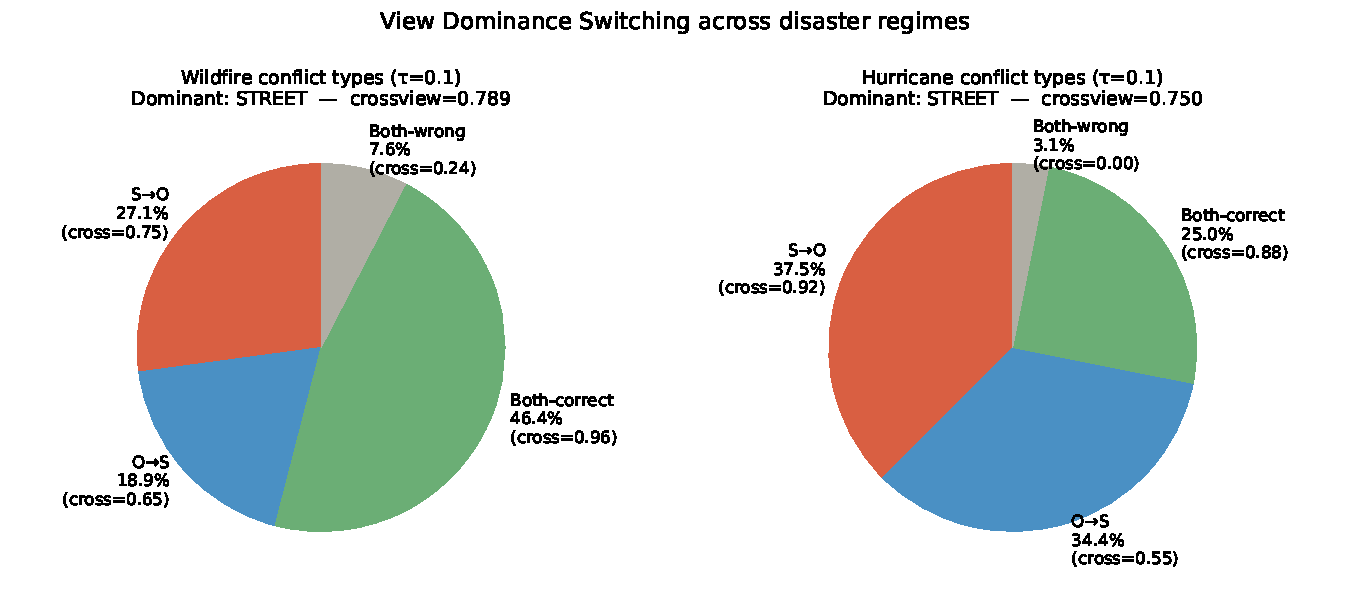
\includegraphics[width=\columnwidth]{figures/view_dominance_switch_tau0.1.pdf}
  \Description{Two pie charts summarize conflict-type decompositions for wildfire and hurricane under tau equals 0.1. Wildfire shows a larger share of street-correct, remote-wrong cases, while hurricane is closer to balanced.}
  \caption{Conflict-type decomposition under the completed \texttt{tau = 0.1} view-dominance analysis.}
  \label{fig:dominance}
\end{figure}

\subsection{Alignment Proxy Supports the Regime Story}

The segmentation-based alignment proxy reinforces this argument. On the conflict
subset, wildfire images have much higher building visibility and more central
building evidence than hurricane images. Mean building ratio is 0.2684 for
wildfire versus 0.0154 for hurricane, and mean center-building ratio is 0.4101
for wildfire versus 0.0271 for hurricane. This is exactly the regime
distinction the paper seeks to formalize: the property-centric wildfire ground
view more often contains direct target evidence, whereas the hurricane ground
view is much more environment-dominant.

\begin{figure}[t]
  \centering
  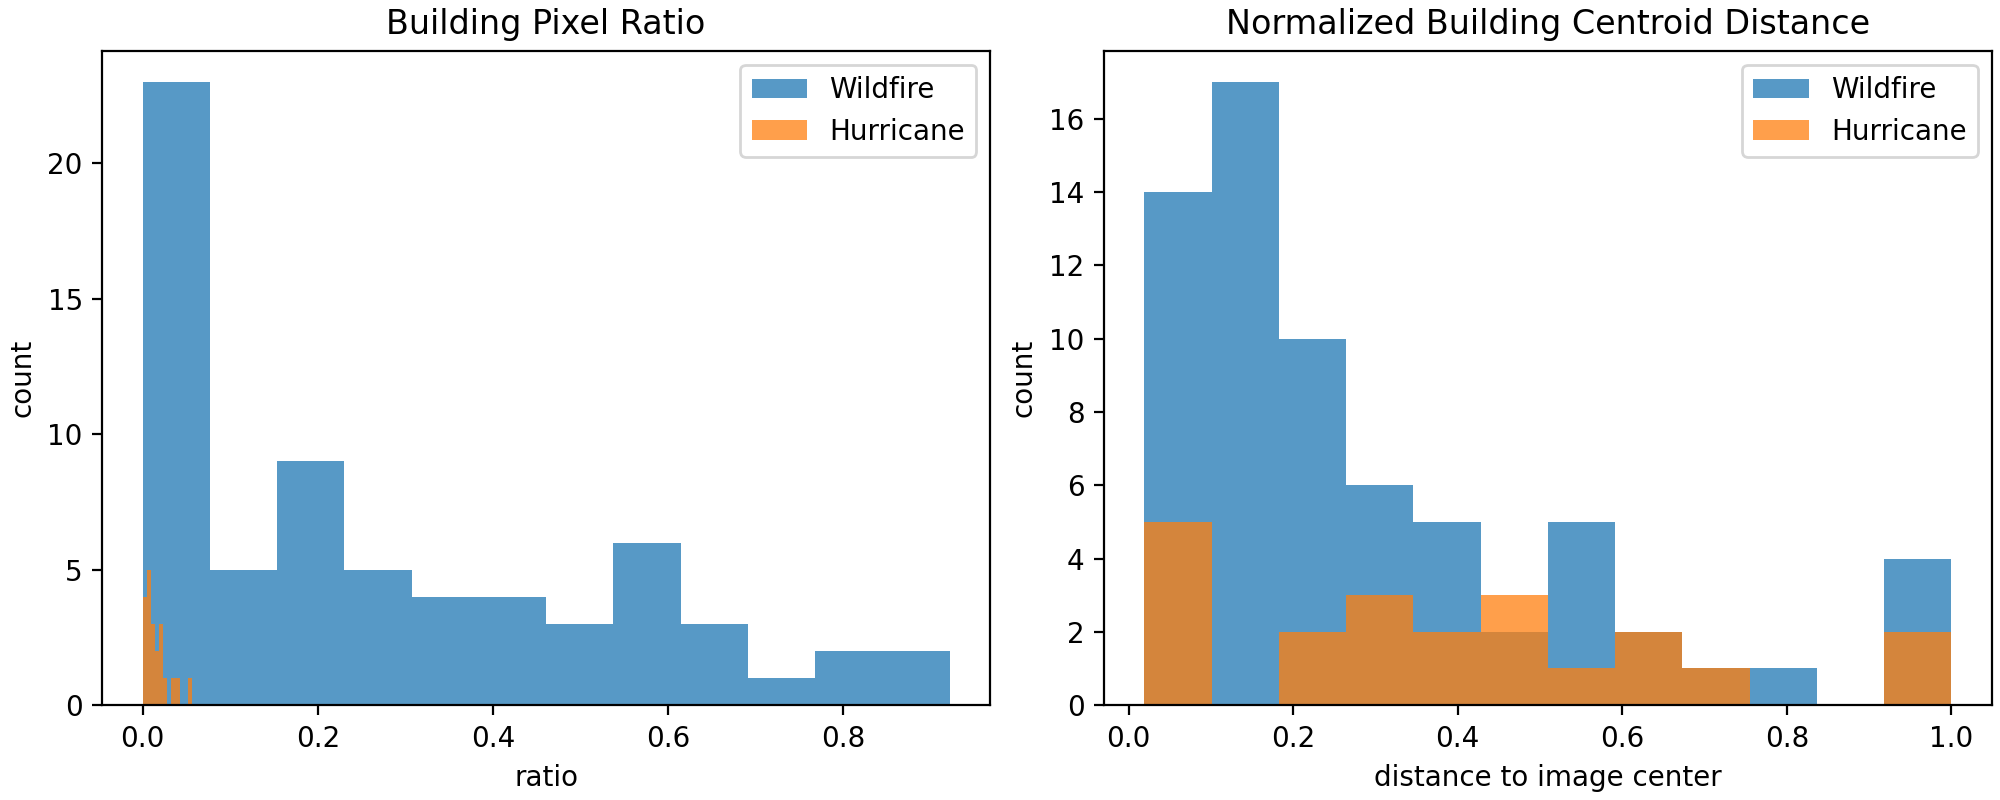
\includegraphics[width=\columnwidth]{figures/building_alignment_comparison.png}
  \Description{A comparison plot contrasts wildfire and hurricane conflict subsets using building ratio, center building ratio, and centroid distance. Wildfire shows higher visible building content and more centered building evidence.}
  \caption{A lightweight alignment proxy suggests much stronger target
  alignment in wildfire conflict images than in hurricane conflict images.}
  \label{fig:alignment}
\end{figure}

\subsection{The Conflict Story Persists Under Softer Thresholds}

The disagreement-centered story remains stable under the \texttt{tau = 0.1}
definition. On that conflict subset, wildfire accuracy is street $= 0.7356$,
remote $= 0.6529$, and crossview $= 0.7885$. For the broader hurricane
sensitivity setting, the corresponding numbers are street $= 0.7031$, remote
$= 0.7266$, and crossview $= 0.7500$, with both permutation tests yielding
\texttt{p < 1e-4}. This confirms that the disagreement-centered effect is not
an artifact of a single hard-threshold definition.

\begin{figure*}[t]
  \centering
  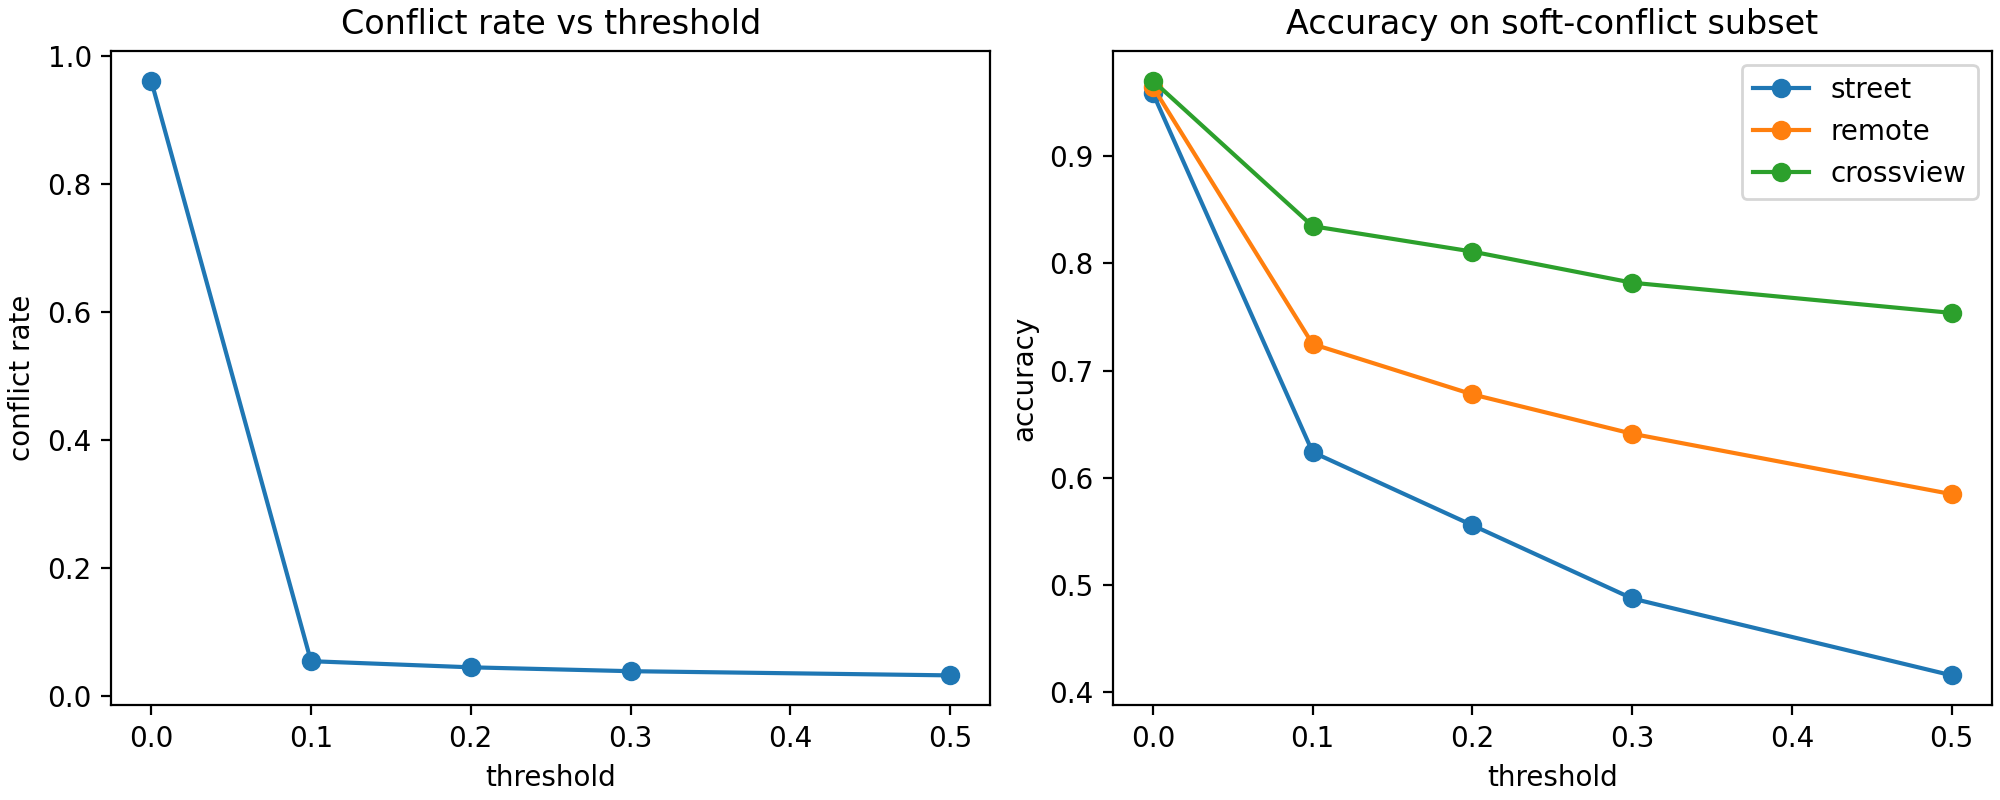
\includegraphics[width=0.48\textwidth]{figures/wildfire_threshold_sensitivity.png}
  \hfill
  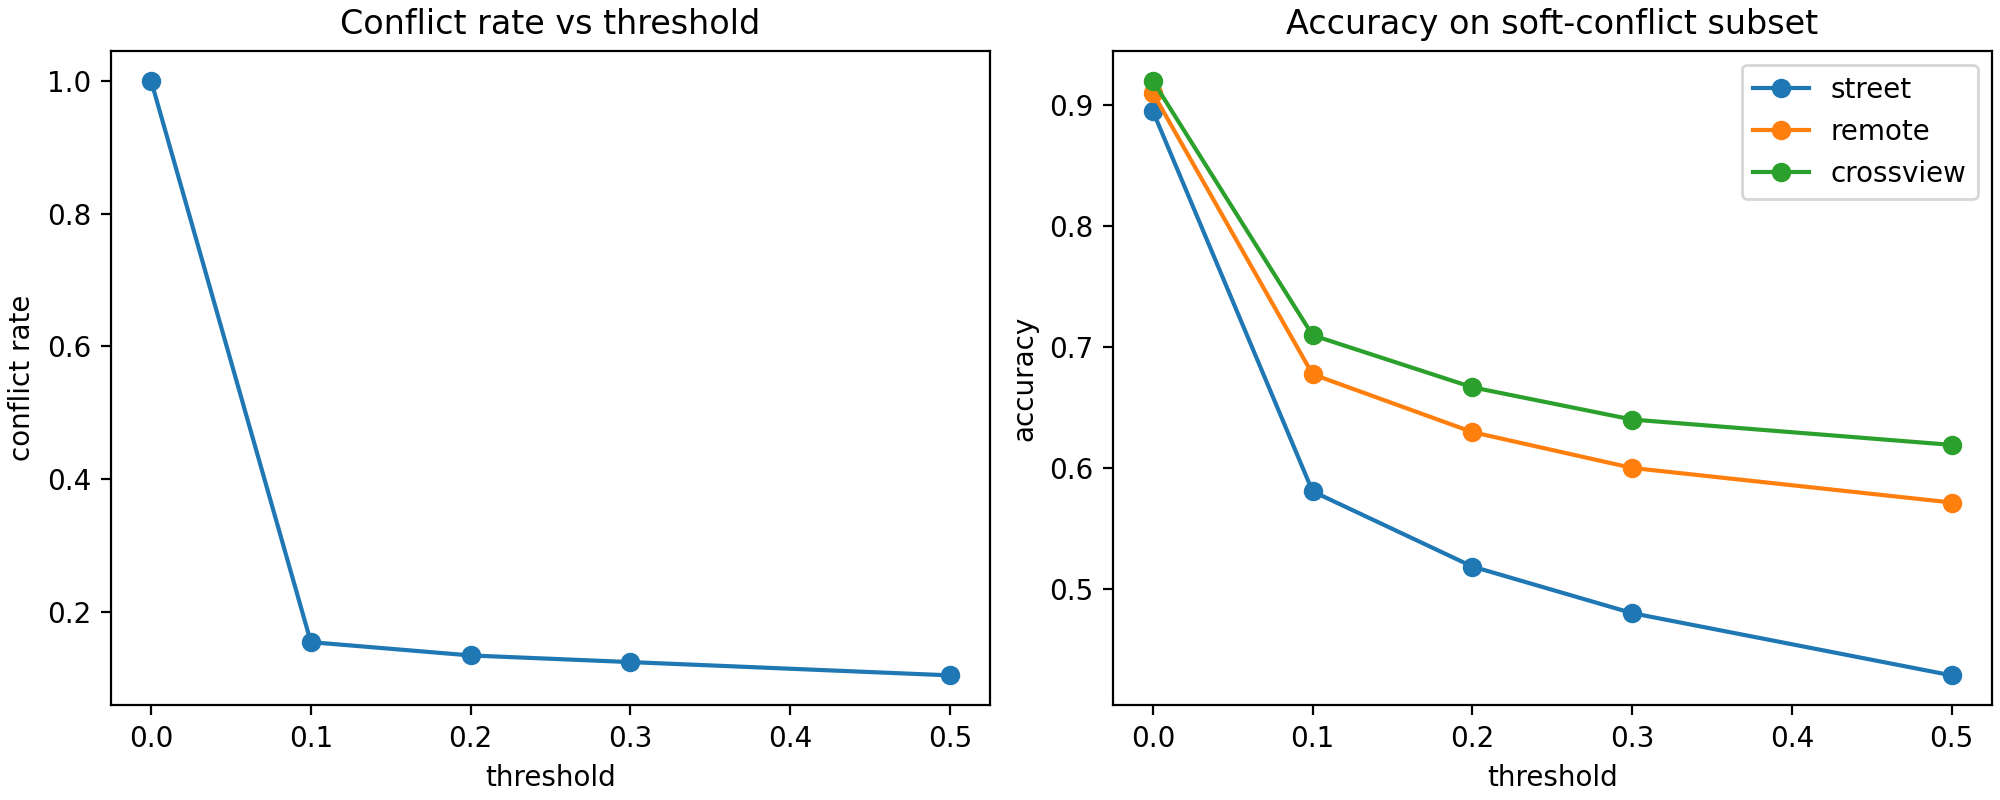
\includegraphics[width=0.48\textwidth]{figures/hurricane_threshold_sensitivity.png}
  \Description{Two threshold-sensitivity plots show that crossview remains the strongest or near-strongest configuration as the disagreement threshold varies, for wildfire on the left and hurricane on the right.}
  \caption{Threshold sensitivity under softer and harder conflict definitions. The conflict-aware story is not tied to a single threshold choice.}
  \label{fig:threshold}
\end{figure*}

\subsection{Backbone and Multi-Seed Robustness}

The backbone results show that larger or more generic pretraining is not
automatically better for cross-view disaster triage. On wildfire crossview,
best validation F1 is 0.9676 for ResNet18, 0.9693 for ResNet50, 0.9378 for
DINOv2, and 0.7502 for CLIP. On hurricane crossview, the corresponding values
are 0.9694, 0.9470, 0.7975, and 0.6437. These results strengthen the paper in
two ways: the cross-view pattern is not a tiny-backbone artifact, and generic
vision-language pretraining does not transfer cleanly to this task.

The main pattern is also stable across seeds. Wildfire multi-seed mean and
standard deviation are 0.9689 $\pm$ 0.0011 for crossview, 0.9657 $\pm$ 0.0001
for street\_only, and 0.9654 $\pm$ 0.0015 for remote\_only. Hurricane
multi-seed values are 0.9455 $\pm$ 0.0063, 0.9433 $\pm$ 0.0012, and
0.8959 $\pm$ 0.0065, respectively.

\subsection{Label Sensitivity and Clean Hurricane Control}

The broader hurricane binary mapping remains cross-view favorable:
crossview $= 0.8915$, street\_only $= 0.8738$, and remote\_only $= 0.8873$.
The broader wildfire binary mapping also preserves the ordering:
crossview $= 0.9473$, street\_only $= 0.9392$, and remote\_only $= 0.9238$.
These sensitivity checks matter because they show that the cross-view story is
not limited to one exact label collapse.

After fixing object-level leakage in the hurricane endpoint split, we reran the
core baselines on a clean grouped split. The resulting test F1 values are
crossview $= 0.9008$, street\_only $= 0.9016$, and remote\_only $= 0.8385$.
This is one of the most important sanity checks in the paper because it
prevents overclaiming. The clean split shows that the defensible claim is not
``crossview always dominates.'' Rather, crossview remains useful as a
conflict-aware comparator and clearly outperforms remote-only on the clean
split, while its advantage over street-only can shrink depending on the task
definition and split rigor.

\subsection{ConflictFocalLoss and the Spatial Map Extension}

The complete ConflictFocalLoss sweep on wildfire sensitivity yields:
baseline crossview $= 0.9473$, gamma $= 0.1$ gives 0.9514, gamma $= 0.25$
gives 0.9507, gamma $= 0.5$ gives 0.9520, and gamma $= 1.0$ gives 0.9470.
Moderate conflict-aware weighting is consistently beneficial, while overly
strong weighting collapses back toward baseline-level performance. The best
setting improves the wildfire sensitivity task by +0.0047 F1.

On the wildfire dataset, tile-level conflict density also forms a significant
unsupervised damage proxy: \texttt{n\_tiles = 27}, Spearman
$r = 0.5123$, and $p = 0.0063$. This is a strong GeoAI result because it
converts disagreement between two discriminative models into a spatial damage
map without using tile-level labels at inference time.

\begin{figure}[t]
  \centering
  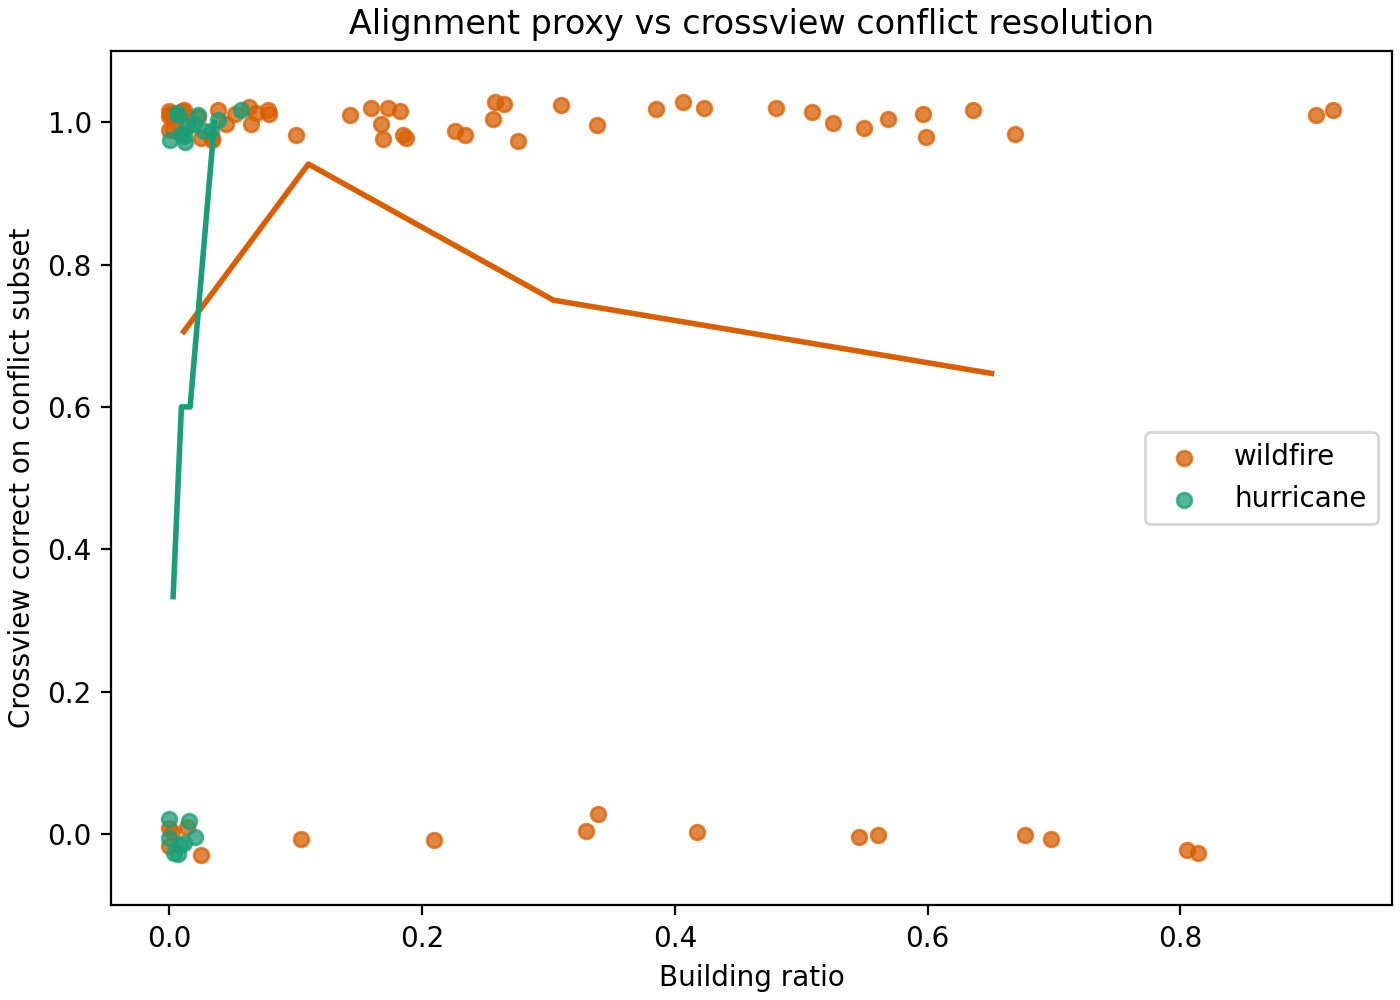
\includegraphics[width=\columnwidth]{figures/alignment_gain_correlation.png}
  \Description{A correlation plot summarizes the relation between building-alignment proxy values and crossview correctness. The trend is weak at the per-sample level, which supports a dataset-level rather than sample-level interpretation.}
  \caption{Per-sample alignment correlation is weak, reinforcing that the
  alignment effect should be interpreted mainly at the regime level.}
  \label{fig:corr}
\end{figure}

\begin{figure*}[t]
  \centering
  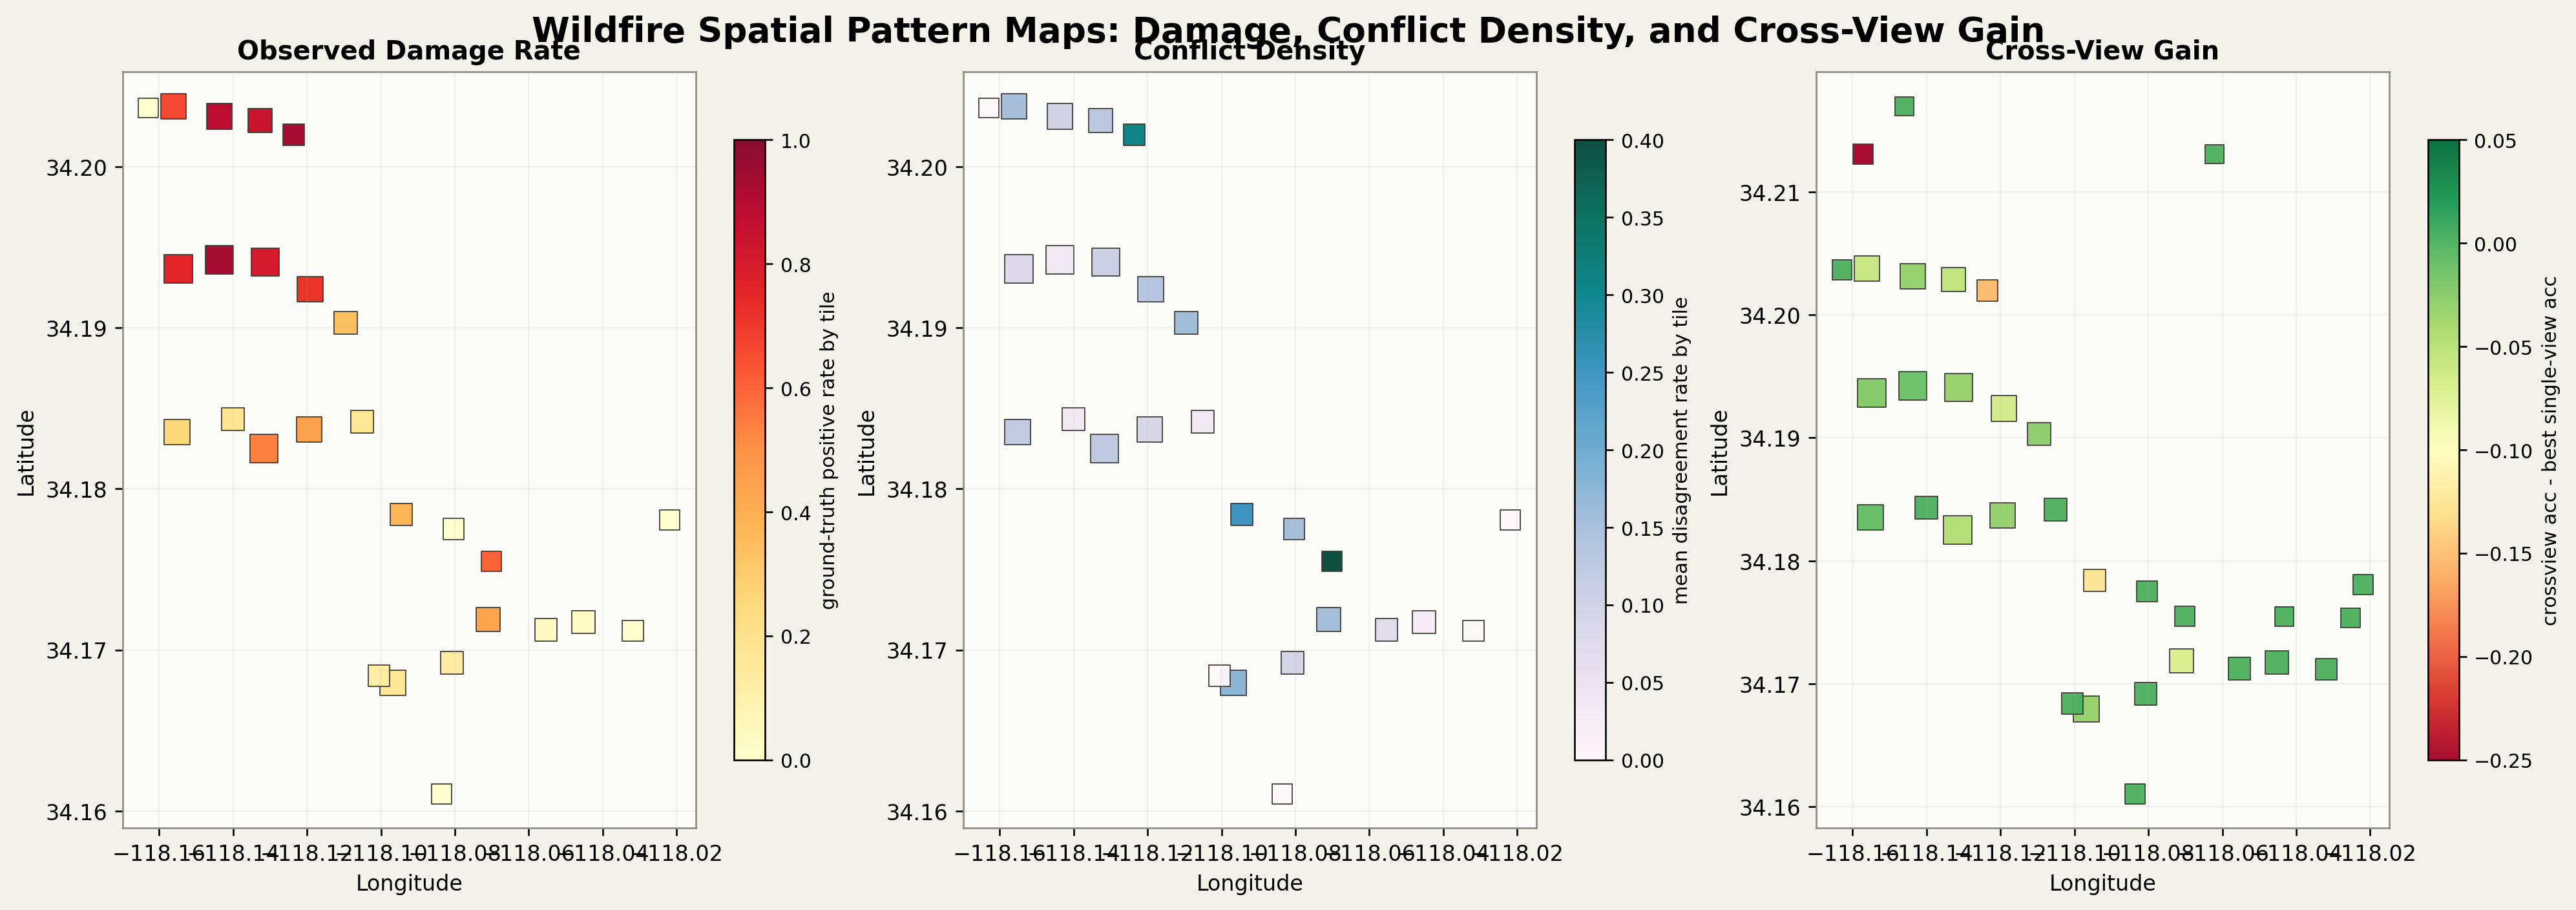
\includegraphics[width=0.9\textwidth]{figures/wildfire_spatial_maps.png}
  \Description{A multi-panel wildfire map compares spatial damage rate, conflict density, and related tile-level analysis outputs. Areas with higher conflict density co-locate with higher damage intensity.}
  \caption{Wildfire conflict-density maps support a tile-level unsupervised
  spatial damage signal.}
  \label{fig:spatialmap}
\end{figure*}

\begin{figure*}[t]
  \centering
  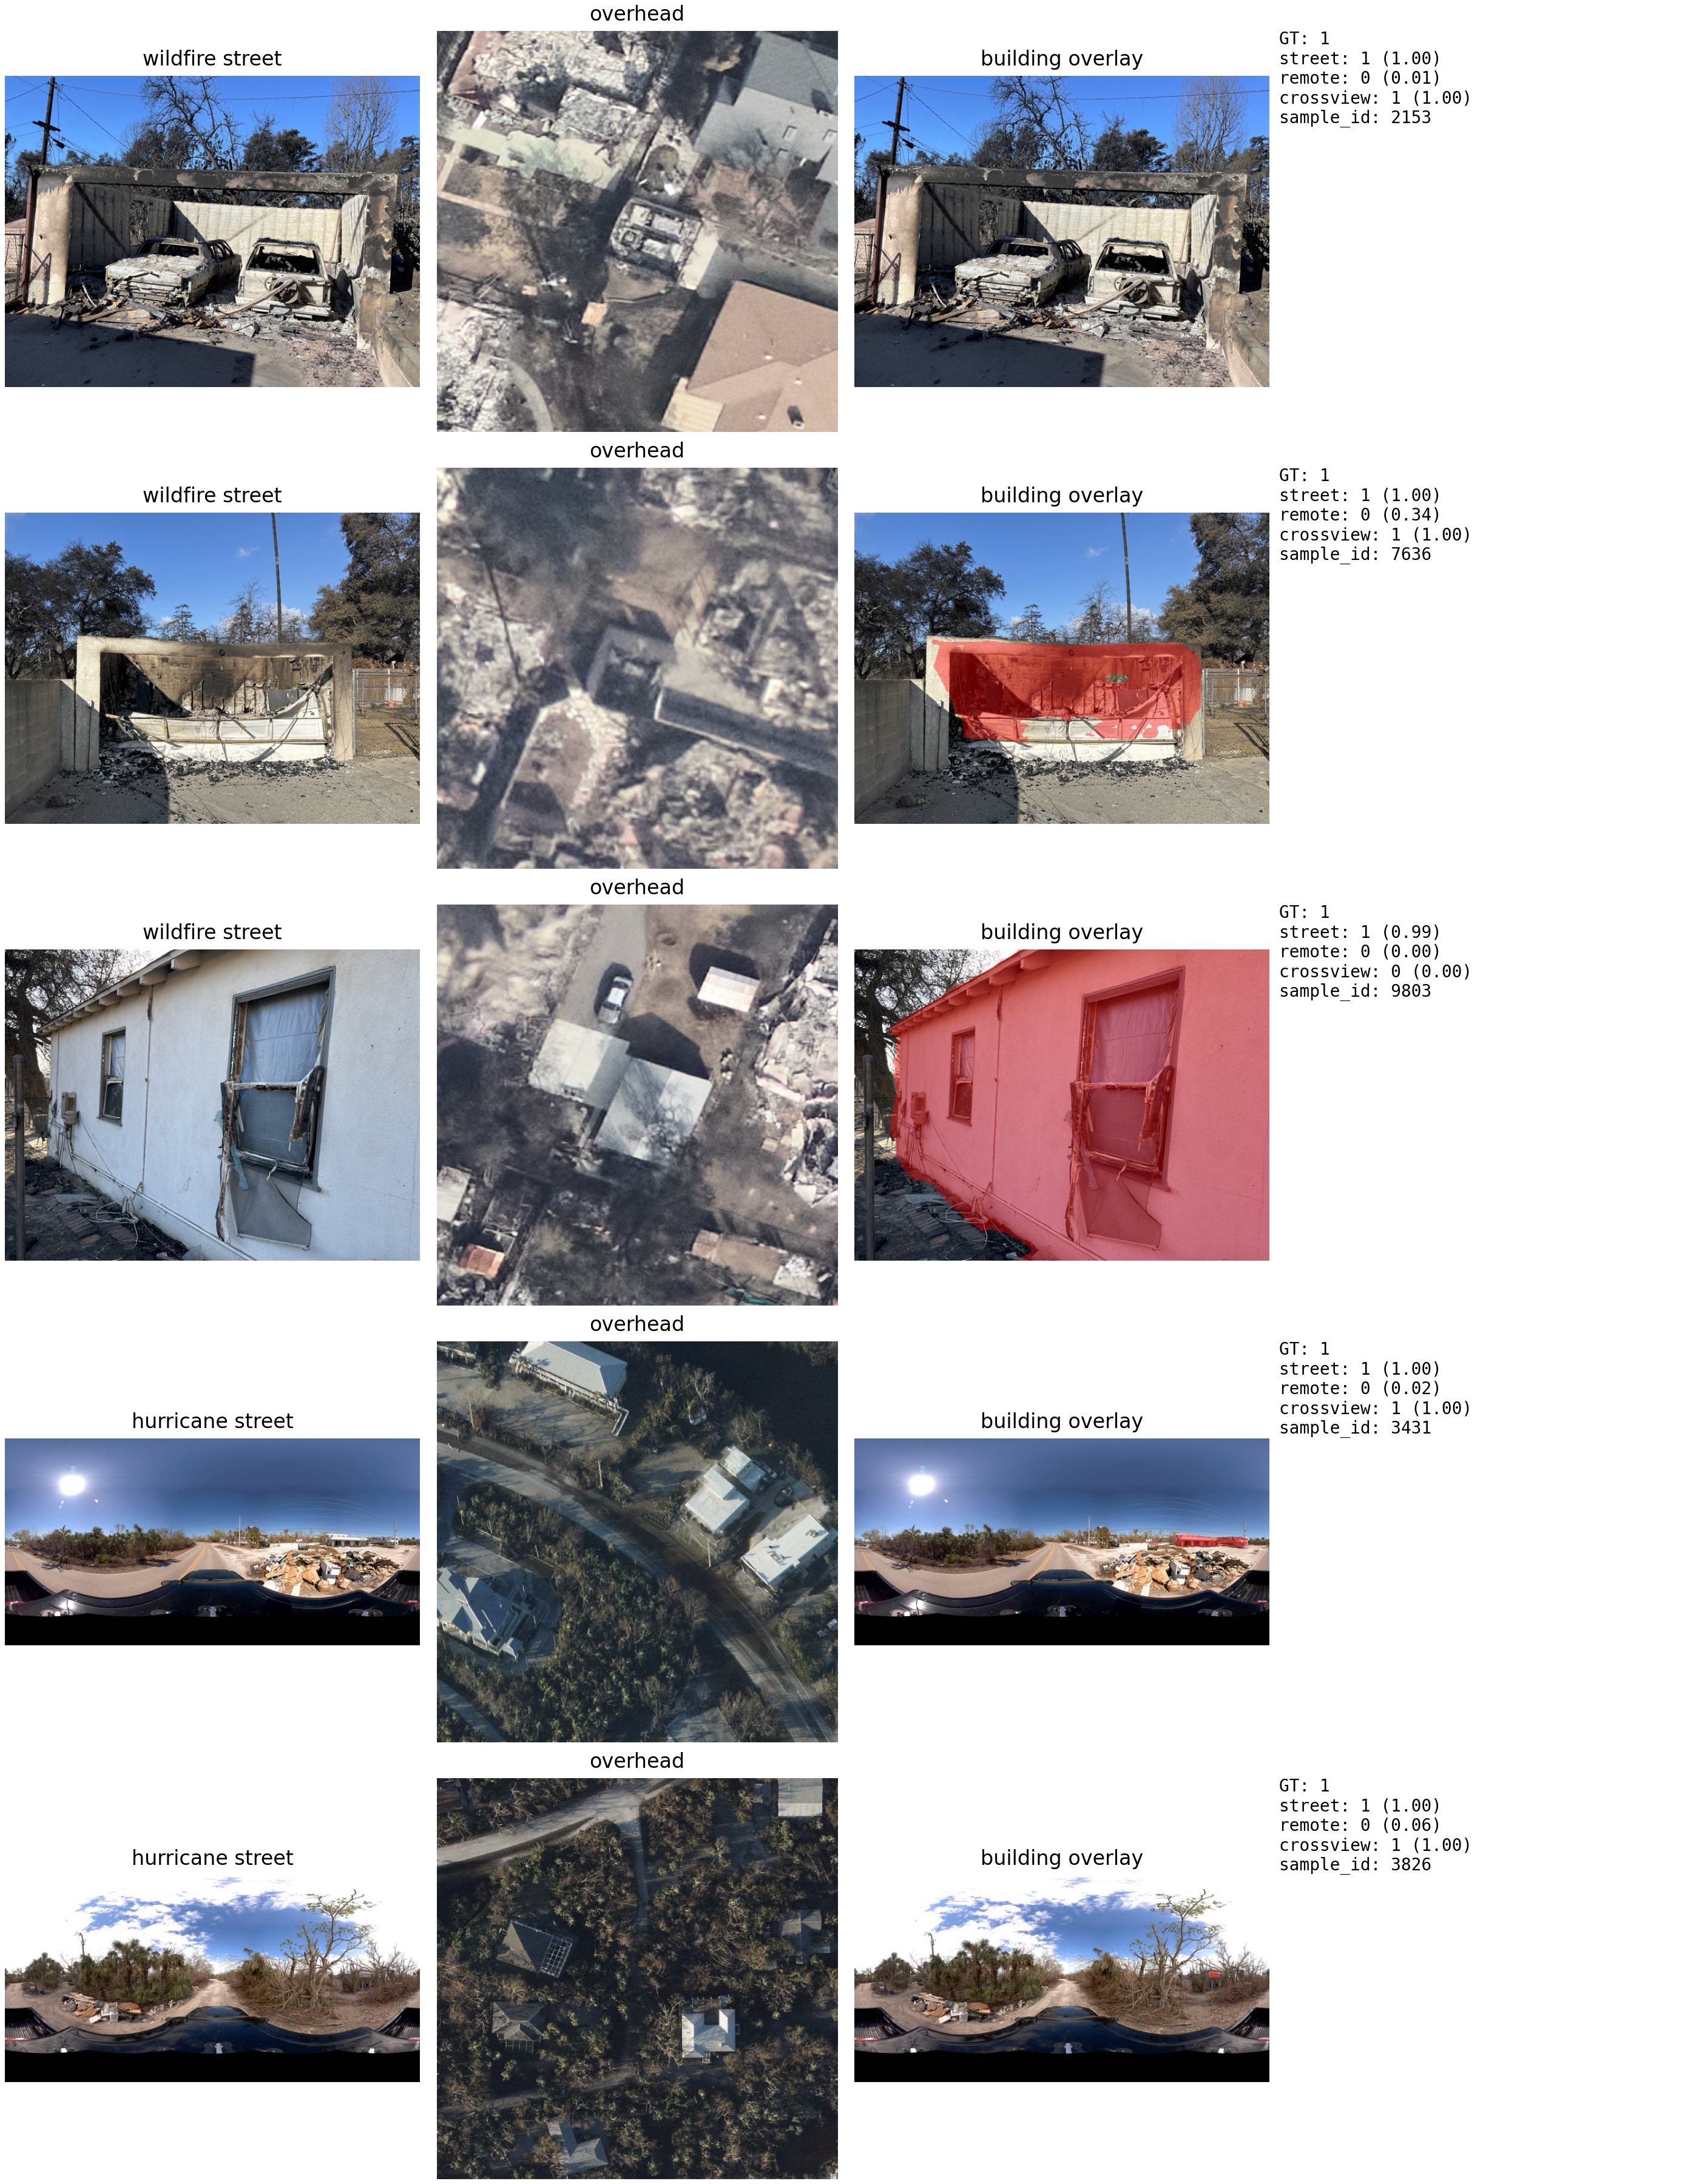
\includegraphics[width=0.92\textwidth]{figures/qualitative_conflict_examples.png}
  \Description{A qualitative figure shows representative conflict cases with ground-view images, overhead patches, and model predictions, highlighting when crossview resolves single-view disagreement.}
  \caption{Qualitative conflict cases. Cross-view fusion is most valuable when
  the two single-view models provide competing evidence.}
  \label{fig:qual}
\end{figure*}

\section{Discussion}

The results support a different way of thinking about cross-view fusion in
disaster intelligence. The main value of fusion is not simply that it adds more
information and nudges up average F1. Its more important function is to resolve
evidence conflict. That is why conflict-centered evaluation is more revealing
than average-case evaluation alone.

The paper also suggests that ``ground-view'' is too coarse a category. A
property-centric inspection image and a panoramic environmental view interact
with overhead imagery in different ways. This is why the paper uses the concept
of spatial observation regime. In one regime, the ground view offers strong
target-specific corrections. In another, the overhead image can remain the more
trustworthy single-view source, or the balance can become split-sensitive
depending on label construction and data leakage control.

This regime-centered explanation is especially relevant for GeoAI. The central
question is not just how to combine modalities, but how the spatial alignment
between the observer and the target changes the utility of each modality. That
framing also creates room for adaptive inference policies, where expensive
cross-view reasoning is reserved for the cases that actually need it.

\section{Limitations}

This paper has several limitations. First, the spatial-map contribution is
currently validated strongly for wildfire but not yet for hurricane, because
the hurricane benchmark does not currently supply equally reliable tile-level
geographic structure for the same analysis. We therefore treat wildfire as the
primary GIS-native spatial analysis dataset and hurricane as a cross-regime
comparison benchmark.

Second, the clean grouped hurricane split leads to a more conservative result
than the original endpoint split. We consider this a strength of the paper's
honesty, but it also means that claims must be phrased carefully. The paper
should emphasize conflict-aware value and regime comparison rather than a
blanket assertion that cross-view always dominates every baseline.

Third, ConflictFocalLoss is currently validated only on the wildfire sensitive
setting. The positive signal is encouraging, but broader validation remains
future work.

\section{Conclusion}

This paper argues that cross-view disaster triage should be understood as
conflict-aware, regime-aware spatial reasoning. Across wildfire and hurricane
paired-view datasets, cross-view fusion is most useful on disagreement cases,
not merely on average cases. The dominant single-view arbitrator changes across
observation regimes and split constructions, which makes conflict-centered
evaluation necessary for honest interpretation. We further show that conflict
can be elevated from an analysis artifact to a method and spatial signal: it
supports conflict-aware training, adaptive cross-view inference, and
unsupervised tile-level damage mapping.

The broader takeaway is that multimodal disaster assessment should not ask only
whether fusion helps. It should ask when fusion helps, which modality drives
the gain, and what spatial regime makes that gain possible.

\bibliographystyle{ACM-Reference-Format}
\bibliography{references}

\end{document}
